\begin{frame}
\frametitle{Scale free graphs as a representation of a social network}

%\begin{itemize}
%\item The transitivity and homophily particularities of social networks gives us guidelines for the parameters for building 
%\end{itemize}

The transitivity and homophily particularities of social networks gives us guidelines for building a scale free graph.


\begin{figure}[H]
\begin{center}
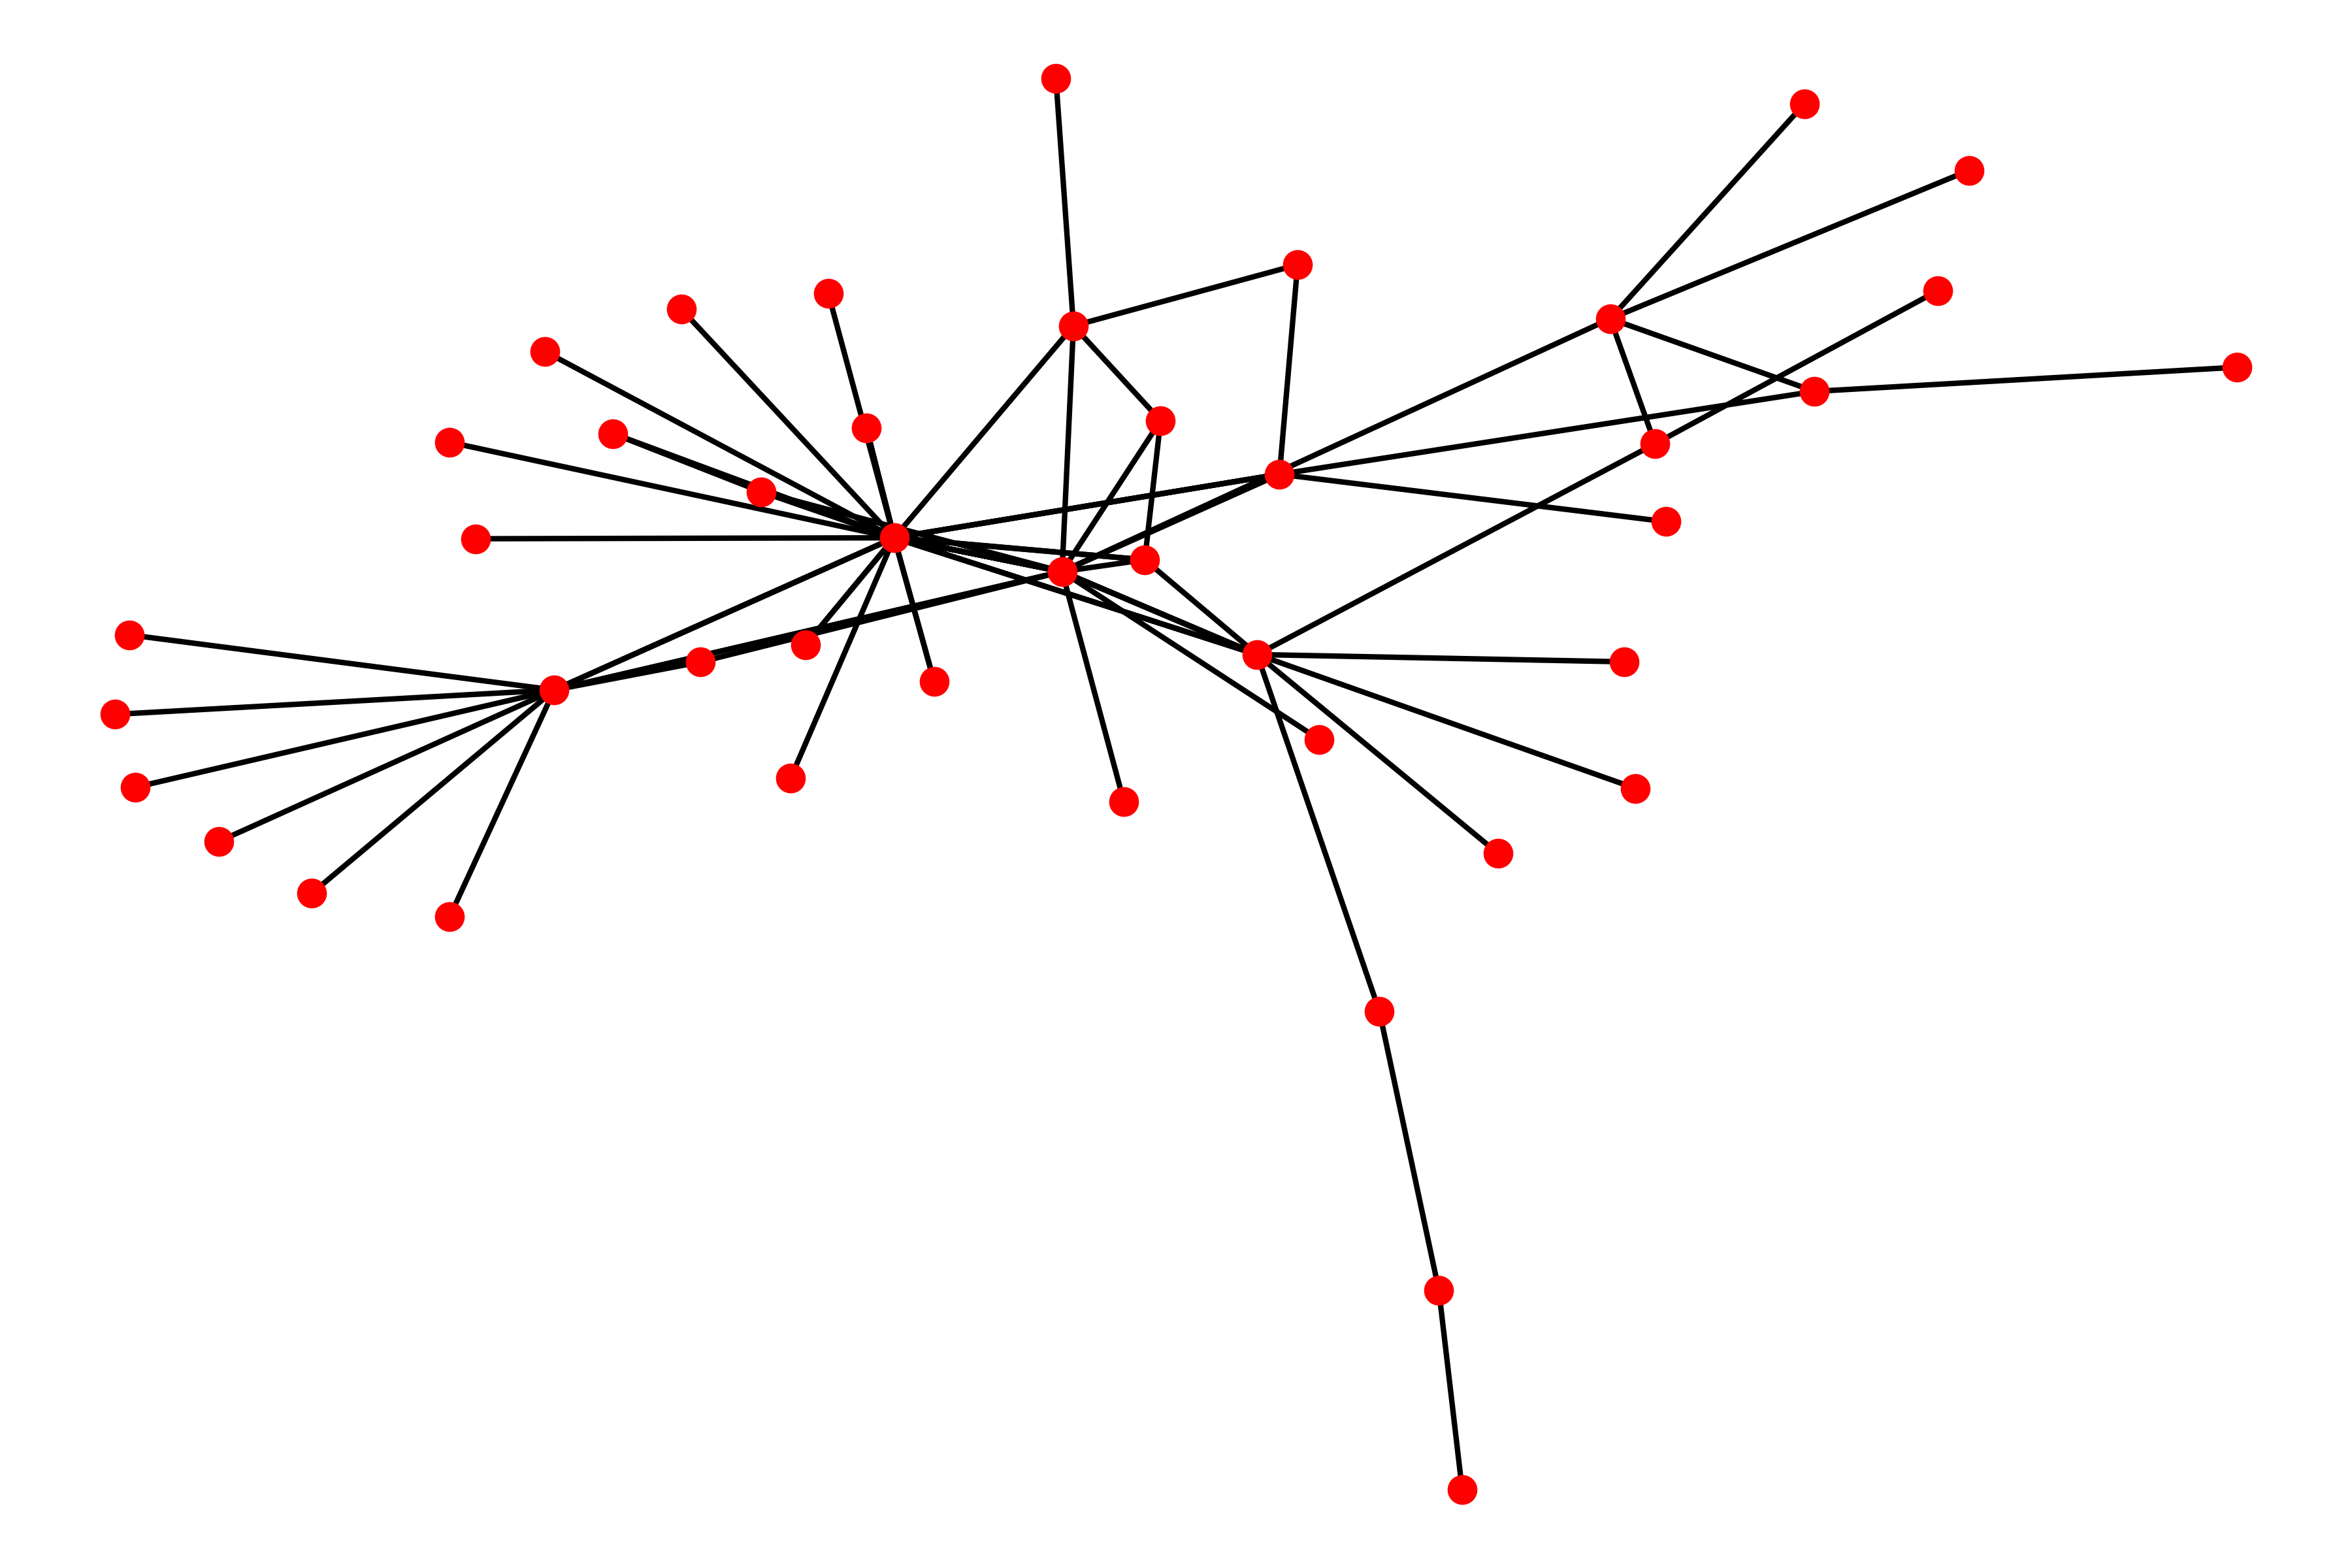
\includegraphics[width=.5\textwidth]{graphScaleFree.png}
\caption{Scale free graph}
\label{fig:ScaleF}
\end{center}
\end{figure}
\end{frame}

% ----------------------------------------------------------------------------------------

\begin{frame}
\frametitle{Results}

\begin{figure}[H]
\begin{center}
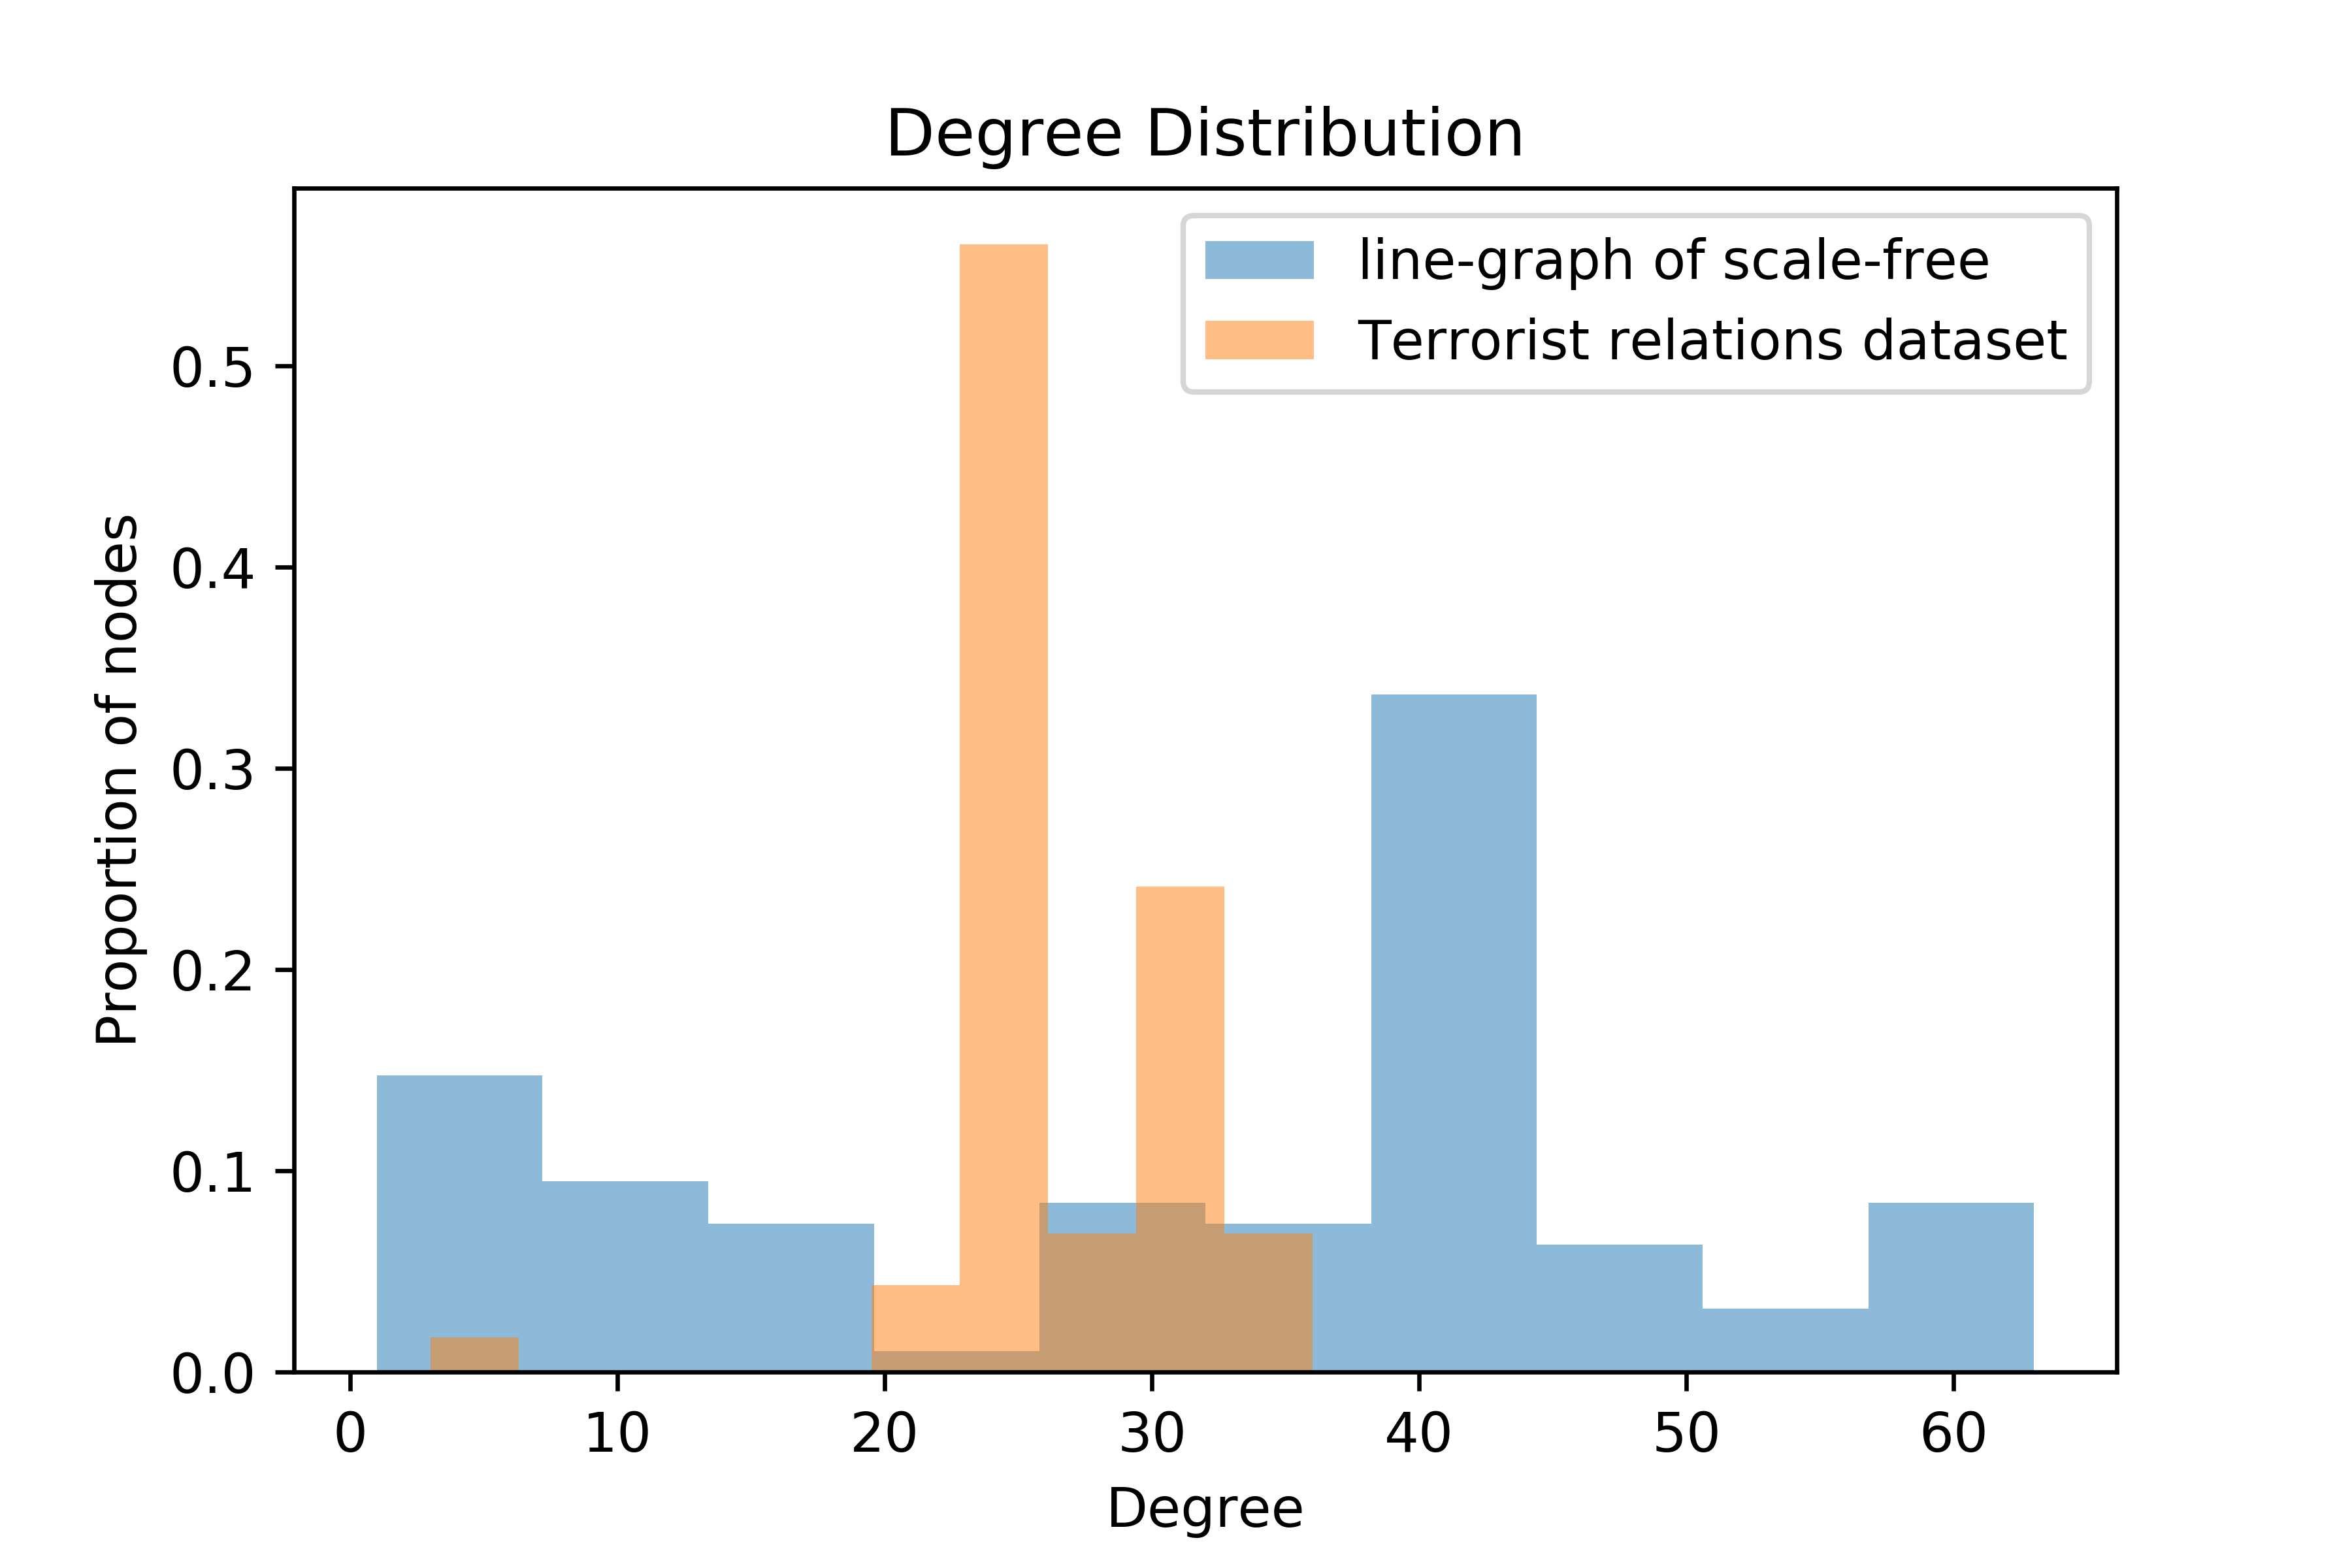
\includegraphics[width=.5\textwidth]{DegreeDiff.png}
\caption{Difference of degree distribution between the dataset and the generated line graph}
\label{fig:degdiff}
\end{center}
\end{figure}

Preliminary conclusion:
\begin{itemize}
\item The relationship network cannot be modeled by the line graph of a scale free network
\item This could be because the relations of terrorist are not similar to social ties
\item This could also be because the size of the largest component is too small
\end{itemize}

\end{frame}